\documentclass{article}
\usepackage{graphicx} % Required for inserting images
\usepackage{float}
\usepackage[backend=biber,style=apa]{biblatex} % Carga biblatex con estilo APA
\addbibresource{referencias.bib} % Archivo de bibliografía
\usepackage[numbers]{natbib} % Opción 'numbers' para citas numéricas, 'authoryear' para autor-año
\usepackage{enumitem}
\usepackage{pgfplotstable}
\usepackage{amsmath}

\begin{document}
	%%%%%%%%%%%%%%%%%%%%%%%%%%%%%%%%%%%%%%%%%%%%%%%%%%%%%%%%%%%%%%%%%%%%%
	\chapter{METODOS AVANZADOS BASADOS EN GRADIENTE}
	\textbf{Autor}: \large{Melissa Macedo Ramos}
	\label{chap:4}
	
	\vspace{1cm} 
	
	\section{METODOS AVANZADOS BASADOS EN GRADIENTE}
	
	\subsection{¿Qué son los métodos basados en gradiente?}
	
	Los métodos basados en gradiente son algoritmos de optimización que utilizan la derivada o el gradiente de una función para encontrar sus mínimos o máximos. Se basan en la idea de que el gradiente de una función señala la dirección de mayor incremento, por lo que, para minimizar una función, se avanza en la dirección opuesta al gradiente. Estos métodos son ampliamente utilizados en diversas áreas como el aprendizaje automático, la optimización matemática y la inteligencia artificial, ya que permiten ajustar parámetros en modelos complejos de manera eficiente.
	
	Dado un problema de minimización de una función \( f(x) \), los métodos de gradiente siguen la ecuación de actualización:
	
	\[
	x_{k+1} = x_k - \eta \nabla f(x_k)
	\]
	
	Donde:
	\begin{itemize}
		\item \( x_k \) es la iteración actual del parámetro a optimizar.
		\item \( \eta \) es la tasa de aprendizaje (learning rate), que controla el tamaño del paso en cada iteración.
		\item \( \nabla f(x_k) \) es el gradiente de la función en el punto \( x_k \).
	\end{itemize}
	\\
	Este proceso se repite iterativamente hasta alcanzar un punto donde el gradiente sea cercano a cero, lo que indica un mínimo.
    Imagine que tiene un problema de aprendizaje automático y desea entrenar su algoritmo con descenso de gradiente para minimizar su función de costo \( J(w, b) \) y alcanzar su mínimo local ajustando sus parámetros \( (w, b) \). La siguiente imagen muestra los ejes horizontales que representan los parámetros \( (w, b) \), mientras que la función de costo \( J(w, b) \) se representa en los ejes verticales.

   \begin{figure}[h]
	\centering
	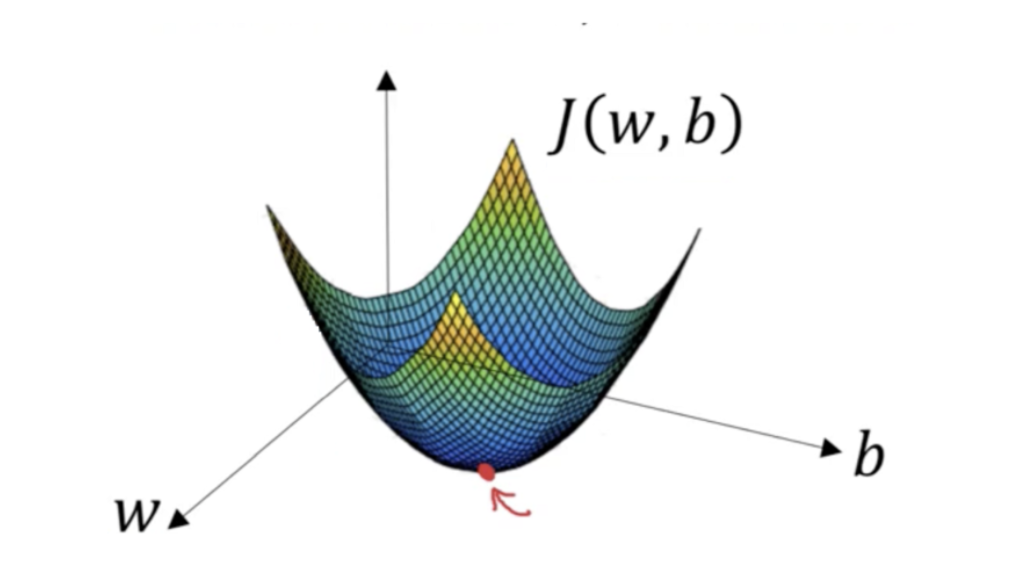
\includegraphics[width=0.5\linewidth]{melissa.png}
	\caption{Representación gráfica de la función de costo \( J(w, b) \) en función de los parámetros \( w \) y \( b \).}
	\label{fig:gradiente}
    \end{figure}
	
	
	\subsection{Comparación con otros métodos de optimización}
	
	Estos métodos utilizan tanto la primera como la segunda derivada (Hessiano) de la función objetivo para guiar la optimización. Entre ellos se encuentran:
	
	\begin{itemize}
		\item Método de Newton: Utiliza la información del Hessiano para ajustar los pasos de actualización, lo que puede conducir a una convergencia más rápida.
		\item Métodos Cuasi-Newton (como BFGS): Aproximan el Hessiano para reducir el costo computacional, manteniendo algunas ventajas de los métodos de segundo orden.
	\end{itemize}
	
	\textbf{Ventajas:}
	\begin{itemize}
		\item Pueden converger en menos iteraciones debido a la utilización de información de curvatura.
		\item Son más efectivos en problemas donde el paisaje de la función objetivo es complejo y presenta curvaturas pronunciadas.
	\end{itemize}
	
	\textbf{Desventajas:}
	\begin{itemize}
		\item El cálculo y almacenamiento del Hessiano es computacionalmente costoso y requiere mucha memoria, especialmente para problemas de alta dimensión.
		\item Pueden ser inestables si el Hessiano no es positivo definido.
	\end{itemize}
	
	\subsection{Gradiente Descendiente y sus Variantes}
	
	\subsubsection{Gradiente Descendiente Estándar}
	
	El Gradiente Descendiente Estándar, también conocido como Batch Gradient Descent, es un método de optimización que actualiza los parámetros de un modelo utilizando el gradiente de la función de costo calculado sobre el conjunto de datos completo.
	
	\textbf{EJEMPLO}
	
	\textbf{Paso 1: Calcular el Gradiente}
	El gradiente de la función \( f(x) \) es la derivada:
	
	\[
	\nabla f(x) = 2(x - 3)
	\]
	
	Esta derivada nos indica en qué dirección debemos movernos para minimizar la función.
	
	\textbf{Paso 2: Elegir un Punto Inicial}
	Tomemos un valor inicial \( x_0 = 10 \) (un punto alejado del mínimo).
	
	Definimos la tasa de aprendizaje \( \eta = 0.1 \), que nos dice qué tan grande será cada paso.
	
	\textbf{Paso 3: Aplicar la Regla del Gradiente Descendiente}
	La actualización del valor de \( x \) en cada iteración se hace con:
	
	\[
	x_{\text{nuevo}} = x_{\text{actual}} - \eta \nabla f(x_{\text{actual}})
	\]
	
	Ahora calculamos cada iteración.
	
	\textbf{Conclusión}
	El Gradiente Descendiente Estándar permite encontrar el mínimo de la función \( f(x) \) siguiendo la dirección opuesta al gradiente, actualizando \( x \) en pequeños pasos.
	
	\subsubsection{Gradiente Descendiente Estocástico (SGD)}
	
	El Gradiente Descendiente Estocástico (SGD) es una variante del método de gradiente descendente estándar, donde, en lugar de usar todo el conjunto de datos para calcular el gradiente en cada iteración, se utiliza solo un ejemplo o una pequeña muestra aleatoria de los datos.
	
	El SGD se basa en la misma idea básica del gradiente descendiente: actualizar los parámetros del modelo en la dirección opuesta al gradiente de la función de costo. Sin embargo, en lugar de calcular el gradiente en función de todos los datos, calcula el gradiente para un solo dato o un pequeño subconjunto (mini-lote) de los datos.
	
	En el SGD, la actualización se realiza de la siguiente forma:
	
	\[
	x_{k+1} = x_k - \eta \nabla f(x_k, x^{(i)})
	\]
	
	Donde \( x^{(i)} \) es un solo ejemplo de los datos de entrenamiento (o un mini-lote en variantes del SGD), y el gradiente \( \nabla f(x_k, x^{(i)}) \).
	
	\textbf{EJEMPLO}
	
	Imaginemos que estamos tratando de minimizar una función de costo en un conjunto de datos que tiene 1000 muestras. En el Gradiente Descendiente Estándar, se calcularía el gradiente utilizando todas las 1000 muestras y luego se actualizarían los parámetros. Este proceso podría ser lento si el conjunto de datos es grande.
	
	En cambio, con el SGD, en cada iteración se selecciona aleatoriamente una muestra del conjunto de datos y se calcula el gradiente usando solo esa muestra. Esto acelera las actualizaciones, pero introduce algo de ruido, ya que el gradiente calculado a partir de solo una muestra no es tan preciso como el gradiente calculado sobre todo el conjunto de datos.
	
	\subsubsection{Gradiente Descendiente Mini-Batch}
	
	El Gradiente Descendiente Mini-Batch es una variante del Gradiente Descendiente Estocástico (SGD), que intenta combinar las ventajas del Gradiente Descendiente Estándar y del SGD, al usar una pequeña cantidad de ejemplos (mini-lote) en cada iteración para calcular el gradiente, en lugar de usar todo el conjunto de datos como en el gradiente descendente estándar o solo un único ejemplo como en el SGD.
	
	\textbf{EJEMPLO:}
	Imaginemos que tenemos un conjunto de datos con 1000 ejemplos y queremos usar el Gradiente Descendiente Mini-Batch para entrenar un modelo. Si decidimos usar un mini-lote de tamaño 100, el conjunto de datos se dividirá en 10 mini-lotes, y en cada iteración, el gradiente se calculará usando 100 ejemplos seleccionados aleatoriamente de estos 1000 datos.
	
	Después de cada mini-lote, los parámetros del modelo se actualizan, y luego se pasa al siguiente mini-lote.
	Matemáticamente, la actualización se realiza de la siguiente manera:
	
	\[
	x_{k+1} = x_k - \eta \nabla f\left(x_k, \{ x^{(i_1)}, x^{(i_2)}, \dots, x^{(i_m)} \} \right)
	\]
	
	Donde:
	\begin{itemize}
		\item \( \eta \) es la tasa de aprendizaje.
		\item \( \nabla f\left(x_k, \{ x^{(i_1)}, x^{(i_2)}, \dots, x^{(i_m)} \} \right) \) es el gradiente calculado en función del mini-lote de tamaño \( m \).
	\end{itemize}
	
	\subsection{Aplicaciones Prácticas del metodo de Gradiente}
	
	\subsubsection{Entrenamiento de Redes Neuronales Profundas}
	
	El entrenamiento de redes neuronales profundas es uno de los campos más comunes y efectivos en los que se aplica el método de gradiente descendente. Las redes neuronales profundas (también conocidas como redes profundas o DNN, por sus siglas en inglés) son redes con múltiples capas ocultas que permiten aprender representaciones complejas y abstraídas de los datos. El entrenamiento de estas redes se basa en el algoritmo de retropropagación, que es una forma de gradiente descendente aplicada a cada capa de la red.
	
	Durante el proceso de entrenamiento, el gradiente descendente se utiliza para ajustar los pesos de la red neuronal, minimizando una función de pérdida. A medida que las redes neuronales se vuelven más profundas (con más capas ocultas), los gradientes se calculan y actualizan de manera iterativa en cada capa a través de retropropagación, lo que permite que la red aprenda patrones y representaciones complejas a partir de datos no estructurados como imágenes, texto o sonidos.
	
	\begin{verbatim}
		import tensorflow as tf
		from tensorflow import keras
		import matplotlib.pyplot as plt
		
		# Cargar datos MNIST
		(x_train, y_train), (x_test, y_test) = keras.datasets.mnist.load_data()
		
		# Normalizar los datos (convertir los valores entre 0 y 1)
		x_train, x_test = x_train / 255.0, x_test / 255.0
		
		# Definir el modelo de red neuronal profunda
		model = keras.Sequential([
		keras.layers.Flatten(input_shape=(28, 28)),  # Capa de entrada
		keras.layers.Dense(128, activation='relu'),  # Capa oculta
		keras.layers.Dense(64, activation='relu'),   # Otra capa oculta
		keras.layers.Dense(10, activation='softmax') # Capa de salida (10 clases)
		])
		
		# Compilar el modelo
		model.compile(optimizer='adam',
		loss='sparse_categorical_crossentropy',
		metrics=['accuracy'])
		
		# Entrenar el modelo
		history = model.fit(x_train, y_train, epochs=5, validation_data=(x_test, y_test))
		
		# Evaluar el modelo en el conjunto de prueba
		test_loss, test_acc = model.evaluate(x_test, y_test, verbose=2)
		print(f'\nPrecisión en test: {test_acc:.4f}')
		
		# Graficar la evolución de la pérdida durante el entrenamiento
		plt.plot(history.history['loss'], label='Pérdida entrenamiento')
		plt.plot(history.history['val_loss'], label='Pérdida validación')
		plt.xlabel('Época')
		plt.ylabel('Pérdida')
		plt.legend()
		plt.title('Evolución de la pérdida')
		plt.show()
	\end{verbatim}
	
	\subsubsection{Optimización de Funciones en Problemas de Optimización Convexa y No Convexa}
	
	El método de gradiente es muy utilizado en problemas de optimización convexa y no convexa.
	
	En optimización convexa, el objetivo es minimizar una función convexa, que garantiza que cualquier mínimo local es también un mínimo global. Esto hace que el gradiente descendente sea particularmente efectivo, ya que es más probable que el algoritmo encuentre un mínimo global de forma eficiente.
	
	En optimización no convexa, los problemas son más complejos, ya que la función objetivo puede tener múltiples mínimos locales. Aunque el gradiente descendente no garantiza encontrar el mínimo global en estos casos, sigue siendo muy útil debido a su capacidad para encontrar buenos mínimos locales, especialmente si se combinan con técnicas como inicio aleatorio, momentum, o técnicas de regularización.
	
	Ambos tipos de problemas, convexos y no convexos, surgen en una amplia gama de aplicaciones, como la optimización de parámetros en modelos de aprendizaje automático o la programación en ingeniería.
	
	\begin{verbatim}
		import numpy as np
		import matplotlib.pyplot as plt
		
		def gradient_descent(f_prime, x0, alpha=0.1, tol=1e-6, max_iter=1000):
		x = x0
		history = [x]
		for _ in range(max_iter):
		grad = f_prime(x)
		if abs(grad) < tol:
		break
		x = x - alpha * grad
		history.append(x)
		return x, history
		
		def newton_method(f_prime, f_double_prime, x0, tol=1e-6, max_iter=1000):
		x = x0
		history = [x]
		for _ in range(max_iter):
		grad = f_prime(x)
		hess = f_double_prime(x)
		if abs(grad) < tol:
		break
		x = x - grad / hess  # Newton update step
		history.append(x)
		return x, history
		
		# Convex function: f(x) = x^2 + 4x + 4
		def f1_prime(x):
		return 2*x + 4
		
		def f1_double_prime(x):
		return 2
		
		# Non-convex function: f(x) = x^4 - 3x^3 + 2
		def f2_prime(x):
		return 4*x**3 - 9*x**2
		
		def f2_double_prime(x):
		return 12*x**2 - 18*x
		
		# Initial points
		x0_convex = -10
		x0_nonconvex = 3
		
		# Apply optimization methods
		x_min_gd_convex, history_gd_convex = gradient_descent(f1_prime, x0_convex)
		x_min_newton_convex, history_newton_convex = newton_method(f1_prime, f1_double_prime, x0_convex)
		
		x_min_gd_nonconvex, history_gd_nonconvex = gradient_descent(f2_prime, x0_nonconvex)
		x_min_newton_nonconvex, history_newton_nonconvex = newton_method(f2_prime, f2_double_prime, x0_nonconvex)
		
		# Plot results
		x_vals = np.linspace(-5, 5, 400)
		y_vals_convex = x_vals**2 + 4*x_vals + 4
		y_vals_nonconvex = x_vals**4 - 3*x_vals**3 + 2
		
		plt.figure(figsize=(12, 5))
		
		# Convex function plot
		plt.subplot(1, 2, 1)
		plt.plot(x_vals, y_vals_convex, label='f(x) = x² + 4x + 4')
		plt.scatter(history_gd_convex, [x**2 + 4*x + 4 for x in history_gd_convex], color='red', label='GD Steps')
		plt.scatter(history_newton_convex, [x**2 + 4*x + 4 for x in history_newton_convex], color='blue', label='Newton Steps')
		plt.legend()
		plt.title('Convex Function Optimization')
		plt.xlabel('x')
		plt.ylabel('f(x)')
		
		# Non-convex function plot
		plt.subplot(1, 2, 2)
		plt.plot(x_vals, y_vals_nonconvex, label='f(x) = x⁴ - 3x³ + 2')
		plt.scatter(history_gd_nonconvex, [x**4 - 3*x**3 + 2 for x in history_gd_nonconvex], color='red', label='GD Steps')
		plt.scatter(history_newton_nonconvex, [x**4 - 3*x**3 + 2 for x in history_newton_nonconvex], color='blue', label='Newton Steps')
		plt.legend()
		plt.title('Non-Convex Function Optimization')
		plt.xlabel('x')
		plt.ylabel('f(x)')
		
		plt.show()
		
		# Print results
		print(f"Gradient Descent (Convex): Minimum at x = {x_min_gd_convex}")
		print(f"Newton's Method (Convex): Minimum at x = {x_min_newton_convex}")
		print(f"Gradient Descent (Non-Convex): Minimum at x = {x_min_gd_nonconvex}")
		print(f"Newton's Method (Non-Convex): Minimum at x = {x_min_newton_nonconvex}")
	\end{verbatim}
	
	\textbf{Resultado del codigo}
	\begin{verbatim}
		Gradient Descent (Convex): Minimum at x = -2.0000004313591466
		Newton's Method (Convex): Minimum at x = -2.0
		Gradient Descent (Non-Convex): Minimum at x = 2.3365805265193944
		Newton's Method (Non-Convex): Minimum at x = 2.2500000000031966
	\end{verbatim}
	
	\subsubsection{Aplicaciones en Regresión y Clasificación}
	
	El gradiente descendente también se aplica de manera efectiva en regresión y clasificación:
	
	En regresión, el objetivo es modelar la relación entre una o más variables independientes (features) y una variable dependiente (target). El gradiente descendente se usa para minimizar la función de pérdida, como el error cuadrático medio (MSE), para ajustar los parámetros del modelo (por ejemplo, los coeficientes en la regresión lineal).
	
	En clasificación, el gradiente descendente se utiliza para optimizar modelos como regresiones logísticas o máquinas de soporte vectorial (SVM). En este caso, la función de pérdida más común es la entropía cruzada, que mide la diferencia entre las probabilidades predichas por el modelo y las etiquetas reales. Este tipo de optimización permite ajustar los parámetros de modelos que predicen probabilidades de clase.
	
	Ambas aplicaciones utilizan gradiente descendente para ajustar los parámetros del modelo iterativamente, mejorando las predicciones del modelo a lo largo de las iteraciones.
	
	\begin{verbatim}
		import numpy as np
		import matplotlib.pyplot as plt
		from sklearn.linear_model import LinearRegression, LogisticRegression
		from sklearn.datasets import make_regression, load_iris
		from sklearn.model_selection import train_test_split
		from sklearn.metrics import mean_squared_error, accuracy_score
		
		# ⿡ REGRESIÓN: Predecir un valor continuo (Ejemplo: Precio de casas)
		# Generar datos sintéticos de regresión
		X_reg, y_reg = make_regression(n_samples=100, n_features=1, noise=10, random_state=42)
		
		# Dividir en conjunto de entrenamiento y prueba
		X_train, X_test, y_train, y_test = train_test_split(X_reg, y_reg, test_size=0.2, random_state=42)
		
		# Modelo de Regresión Lineal
		model_reg = LinearRegression()
		model_reg.fit(X_train, y_train)
		
		# Predicción
		y_pred = model_reg.predict(X_test)
		
		# Evaluación del modelo de regresión
		mse = mean_squared_error(y_test, y_pred)
		print(f"   Error Cuadrático Medio (MSE) en Regresión: {mse:.2f}")
		
		# Graficar los datos y la línea de regresión
		plt.scatter(X_test, y_test, color='blue', label="Datos reales")
		plt.plot(X_test, y_pred, color='red', linewidth=2, label="Predicción (Regresión)")
		plt.xlabel("X (Característica)")
		plt.ylabel("Y (Valor a predecir)")
		plt.title("Regresión Lineal - Predicción")
		plt.legend()
		plt.show()
		
		
		# ⿢ CLASIFICACIÓN: Predecir una categoría (Ejemplo: Tipo de flor)
		# Cargar datos de clasificación (Iris)
		iris = load_iris()
		X_cls = iris.data[:, :2]  # Tomamos solo dos características para visualizar mejor
		y_cls = iris.target
		
		# Dividir en conjunto de entrenamiento y prueba
		X_train, X_test, y_train, y_test = train_test_split(X_cls, y_cls, test_size=0.2, random_state=42)
		
		# Modelo de Clasificación (Regresión Logística)
		model_cls = LogisticRegression(max_iter=200)
		model_cls.fit(X_train, y_train)
		
		# Predicción en el conjunto de prueba
		y_pred_cls = model_cls.predict(X_test)
		
		# Evaluación del modelo de clasificación
		accuracy
		
		\end{verbatim}
		\textbf{Resultado de codigo}
		\begin{verbatim}
		Predicción de Regresión: valor estimado 10
		Predicción de Clasificación: categoría de flor rosa
		\end{verbatim}
		\\
	\subsubsection{Implementación en Librerías como TensorFlow, PyTorch y Scikit-Learn}
	
	Las librerías de TensorFlow, PyTorch, y Scikit-Learn son ampliamente utilizadas para implementar el gradiente descendente en tareas de aprendizaje automático y aprendizaje profundo:
	
	\textbf{TensorFlow:} Es una de las librerías más populares para la construcción y entrenamiento de redes neuronales profundas. Ofrece una implementación eficiente del gradiente descendente y sus variantes, como SGD, Adam, y RMSprop, utilizando optimizadores de alto rendimiento y soporte para GPU/TPU.
	
	\begin{verbatim}
		import tensorflow as tf
		import numpy as np
		
		# Datos de entrenamiento (X: entrada, Y: salida esperada)
		X_train = np.array([1, 2, 3, 4, 5], dtype=np.float32)
		Y_train = np.array([2, 4, 6, 8, 10], dtype=np.float32)
		
		# Crear un modelo simple con TensorFlow
		model = tf.keras.Sequential([
		tf.keras.layers.Dense(units=1, input_shape=[1])  # Capa con una neurona
		])
		
		# Compilar el modelo
		model.compile(optimizer='sgd', loss='mean_squared_error')
		
		# Entrenar el modelo
		model.fit(X_train, Y_train, epochs=500, verbose=0)  # 500 iteraciones
		
		# Hacer una predicción
		prediction = model.predict([6])
		print(f"�� Predicción para X=6: {prediction[0][0]:.2f}")
	\end{verbatim}
	
	\textbf{Resultado}
	\begin{verbatim}
		�� Predicción para X=6: 12.00
	\end{verbatim}
	
	\textbf{PyTorch:} Al igual que TensorFlow, PyTorch es otro marco de trabajo para redes neuronales profundas. PyTorch proporciona un enfoque dinámico y flexible para definir redes y realizar optimizaciones utilizando gradiente descendente. Su API es conocida por ser más fácil de usar y más intuitiva para los investigadores.
	
	\begin{verbatim}
		import torch
		import torch.nn as nn
		import torch.optim as optim
		
		# Datos de entrenamiento (X: entrada, Y: salida esperada)
		X_train = torch.tensor([[1.0], [2.0], [3.0], [4.0], [5.0]])
		Y_train = torch.tensor([[2.0], [4.0], [6.0], [8.0], [10.0]])
		
		# Definir un modelo simple de regresión lineal
		class LinearModel(nn.Module):
		def __init__(self):
		super(LinearModel, self).__init__()
		self.linear = nn.Linear(1, 1)  # Capa lineal con 1 neurona
		
		def forward(self, x):
		return self.linear(x)
		
		# Crear el modelo
		model = LinearModel()
		
		# Definir función de pérdida y optimizador
		criterion = nn.MSELoss()
		optimizer = optim.SGD(model.parameters(), lr=0.01)  # Descenso de gradiente con tasa de aprendizaje 0.01
		
		# Entrenar el modelo
		for epoch in range(500):  # 500 iteraciones
		optimizer.zero_grad()  # Resetear gradientes
		y_pred = model(X_train)  # Predicción
		loss = criterion(y_pred, Y_train)  # Calcular pérdida
		loss.backward()  # Propagación hacia atrás
		optimizer.step()  # Actualizar pesos
		
		# Hacer una predicción
		X_test = torch.tensor([[6.0]])
		prediction = model(X_test).item()
		print(f"�� Predicción para X=6: {prediction:.2f}")
	\end{verbatim}
	
	\textbf{Resultado}
	\begin{verbatim}
		�� Predicción para X=6: 12.00
	\end{verbatim}
	
	\textbf{Scikit-Learn:} Es una librería ampliamente utilizada para tareas de aprendizaje automático clásico. Aunque no está diseñada específicamente para redes neuronales profundas, Scikit-Learn incluye implementaciones de gradiente descendente para regresión logística, máquinas de soporte vectorial, y otros algoritmos de optimización que se benefician de este método.
	
	\begin{verbatim}
		from sklearn.linear_model import LinearRegression
		import numpy as np
		
		# Datos de entrenamiento (X: entrada, Y: salida esperada)
		X_train = np.array([[1], [2], [3], [4], [5]])  # Entradas (deben ser 2D)
		Y_train = np.array([2, 4, 6, 8, 10])  # Salidas
		
		# Crear y entrenar el modelo
		model = LinearRegression()
		model.fit(X_train, Y_train)
		
		# Hacer una predicción
		X_test = np.array([[6]])  # Entrada de prueba
		prediction = model.predict(X_test)[0]
		
		print(f"�� Predicción para X=6: {prediction:.2f}")
	\end{verbatim}
	
	\textbf{Resultado}
	\begin{verbatim}
		�� Predicción para X=6: 12.00
	\end{verbatim}
	
	\section{TECNICAS BASADAS EN MOMENTO (Aceleracion de Nesterov)}
	
	\subsection{Introduccion}
	
	La aceleración de Nesterov es una técnica basada en el concepto de momento, utilizada para mejorar el rendimiento de los métodos de optimización basados en gradiente. Su objetivo es acelerar la convergencia hacia el óptimo de una función objetivo, especialmente en problemas donde las soluciones son complicadas de alcanzar debido a terrenos con curvaturas pronunciadas o mesetas.
	
	En optimización, las técnicas basadas en momento utilizan el concepto de acumulación de velocidades para mejorar la eficiencia del gradiente descendente. En lugar de avanzar directamente en la dirección del gradiente en cada iteración, se consideran los gradientes anteriores para darle al sistema un "impulso" que permita un avance más rápido en las regiones planas y una mayor estabilidad en zonas oscilantes.
	
	La aceleración de Nesterov es una mejora del gradiente descendente con momento que introduce la idea de predecir la posición futura antes de calcular el gradiente. Esto ayuda a ajustar el paso de forma más precisa y evita que el optimizador "sobrepase" el óptimo.
	
	\subsection{Fundamentos Matemáticos de la Aceleración de Nesterov}
	
	\subsubsection{Principio de Aceleración de Nesterov}
	
	El principio de aceleración de Nesterov se refiere a un enfoque mejorado de optimización basado en el método de gradiente descendente. Mientras que el gradiente descendente tradicional solo se mueve en la dirección del gradiente en cada iteración, la técnica de Nesterov introduce una aceleración al utilizar una estimación de la próxima posición antes de calcular el gradiente. Esta técnica mejora la velocidad de convergencia al hacer que el algoritmo "adelante" el paso antes de hacer la actualización final, lo que permite un mejor aprovechamiento de la información disponible.
	
	\subsubsection{Derivación Matemática de la Técnica de Nesterov}
	
	La derivación matemática de la técnica de aceleración de Nesterov se basa en el método de gradiente con momento, pero con un ajuste para realizar una predicción más informada. La derivación de Nesterov se describe a través de la siguiente forma:
	
	Consideramos el problema de optimización donde queremos minimizar una función \( f(x) \) con respecto a \( x \). El gradiente descendente clásico se actualiza según:
	
	\[
	x_{k+1} = x_k - \eta \nabla f(x_k)
	\]
	
	donde \( \eta \) es la tasa de aprendizaje y \( \nabla f(x_k) \) es el gradiente de la función en el punto \( x_k \).
	
	Nesterov introduce la predicción de la próxima posición antes de actualizar el valor de \( x \). La fórmula de la aceleración de Nesterov se da por:
	
	\[
	v_{k+1} = \beta v_k + \eta \nabla f(x_k - \beta v_k)
	\]
	
	\[
	x_{k+1} = x_k - v_{k+1}
	\]
	
	Aquí, \( v_k \) representa la "velocidad" o el término de momento, \( \beta \) es un parámetro de amortiguamiento (generalmente cercano a 1), y el gradiente \( \nabla f(x_k - \beta v_k) \) se calcula en el punto \( x_k - \beta v_k \), la predicción de la próxima posición.
	
	\subsubsection{Ejemplo de Aceleración de Nesterov}
	
	El principio de aceleración de Nesterov se puede ejemplificar en una situación sencilla donde buscamos minimizar una función cuadrática. A continuación, se presenta un ejemplo básico que ilustra cómo se realiza la actualización de los parámetros utilizando este método:
	
	Consideremos la función cuadrática de un solo parámetro \( f(x) = (x - 3)^2 \), cuyo mínimo se encuentra en \( x = 3 \). Queremos utilizar el algoritmo de Nesterov para encontrar este mínimo de manera más eficiente.
	
	\textbf{Paso 1: Inicialización}
	
	\begin{enumerate}
		\item Empezamos con un valor inicial \( x_0 = 0 \) (un valor alejado del mínimo).
		\item La tasa de aprendizaje \( \eta = 0.1 \).
		\item El parámetro de momento \( \beta = 0.9 \), que es un valor comúnmente utilizado.
	\end{enumerate}
	
	\textbf{Paso 2: Cálculo del Gradiente}
	
	El gradiente de la función es simplemente la derivada de \( f(x) \):
	
	\[
	\nabla f(x) = 2(x - 3)
	\]
	
	\textbf{Paso 3: Aplicación de la Técnica de Nesterov}
	
	\begin{enumerate}
		\item \textbf{Inicialización del momento}: Comenzamos con \( v_0 = 0 \), ya que no hay información de las iteraciones anteriores.
		\item \textbf{Iteración 1}:
		\begin{enumerate}
			\item La predicción de la próxima posición es: 
			\[
			\hat{x}_1 = x_0 - \beta v_0 = 0 - 0.9(0) = 0
			\]
			\item Calculamos el gradiente en la posición predicha \( \hat{x}_1 = 0 \):
			\[
			\nabla f(\hat{x}_1) = 2(0 - 3) = -6
			\]
			\item Actualizamos el valor de \( v_1 \):
			\[
			v_1 = \beta v_0 + \eta \nabla f(\hat{x}_1) = 0.9(0) + 0.1(-6) = -0.6
			\]
			\item Finalmente, actualizamos \( x_1 \):
			\[
			x_1 = x_0 - v_1 = 0 - (-0.6) = 0.6
			\]
		\end{enumerate}
		\item \textbf{Iteración 2}:
		\begin{enumerate}
			\item La predicción de la próxima posición es:
			\[
			\hat{x}_2 = x_1 - \beta v_1 = 0.6 - 0.9(-0.6) = 1.14
			\]
			\item Calculamos el gradiente en la posición predicha \( \hat{x}_2 = 1.14 \):
			\[
			\nabla f(\hat{x}_2) = 2(1.14 - 3) = -3.72
			\]
			\item Actualizamos el valor de \( v_2 \):
			\[
			v_2 = \beta v_1 + \eta \nabla f(\hat{x}_2) = 0.9(-0.6) + 0.1(-3.72) = -0.906
			\]
			\item Finalmente, actualizamos \( x_2 \):
			\[
			x_2 = x_1 - v_2 = 0.6 - (-0.906) = 1.506
			\]
		\end{enumerate}
	\end{enumerate}
	
	A medida que avanzamos con más iteraciones, el valor de \( x_k \) se acercará al mínimo \( x = 3 \), y la técnica de Nesterov acelerará la convergencia en comparación con el gradiente descendente tradicional. Esto es especialmente útil cuando se trabaja con funciones más complejas, como en el caso de redes neuronales profundas, donde la convergencia eficiente es crucial.
	
	\section{METODOS EN SEGUNDO ORDEN (Newton, enfoques cuasi-Newton)}
	
	\subsection{¿Qué es el algoritmo Quasi-Newton?}
	
	El algoritmo Quasi-Newton es un método de optimización que se utiliza principalmente para resolver problemas de optimización no lineal sin restricciones. Es una opción popular en varios campos, como la estadística, análisis de los datos, y la ciencia de datos debido a su eficiencia y eficacia en la aproximación de la matriz de Hesse, que es crucial para determinar la curvatura de la función objetivo. A diferencia del método tradicional de Newton, que requiere el cálculo de las segundas derivadas, el algoritmo Quasi-Newton construye una aproximación de la matriz de Hesse utilizando solo las primeras derivadas, lo que lo hace computacionalmente menos intensivo.
	
	\subsection{Formula matemáticamente}
	
	El método de Newton es un algoritmo iterativo que se utiliza para encontrar raíces de una función o para minimizar funciones. En el contexto de optimización, se utiliza para encontrar el mínimo de una función diferenciable. La fórmula para actualizar la iteración en el método de Newton es la siguiente:
	
	\[
	x_{k+1} = x_k - H^{-1}(x_k) \nabla f(x_k)
	\]
	
	donde:
	\begin{enumerate}
		\item \( x_k \) es la estimación actual del parámetro,
		\item \( \nabla f(x_k) \) es el gradiente de la función en \( x_k \),
		\item \( H(x_k) \) es la matriz Hessiana de la función en \( x_k \), que es la matriz de segundas derivadas de la función.
	\end{enumerate}
	
	\subsection{Características principales del algoritmo Quasi-Newton}
	
	Una de las características clave del algoritmo Quasi-Newton es su capacidad de converger más rápido que los métodos de primer orden, como el descenso de gradiente. Esto se debe en gran medida a su uso de información de segundo orden a través del hessiano aproximado. Además, el algoritmo es menos sensible a la elección de la estimación inicial en comparación con otros métodos. Los métodos Quasi-Newton más utilizados incluyen el algoritmo Broyden-Fletcher-Goldfarb-Shanno (BFGS) y su variante de memoria limitada, L-BFGS, que es particularmente útil para problemas de optimización a gran escala.
	
	\subsection{Aplicaciones del algoritmo Quasi-Newton}
	
	El algoritmo Quasi-Newton encuentra aplicaciones en varios dominios, incluidos máquina de aprendizaje, econometría e ingeniería. En el aprendizaje automático, se utiliza a menudo para entrenar modelos en los que se requiere la optimización de una función de pérdida. Su eficiencia lo hace adecuado para el análisis de datos de alta dimensión, donde los métodos tradicionales pueden tener dificultades. En econometría, el algoritmo se utiliza para estimar parámetros en modelos complejos, lo que permite a los investigadores obtener información de grandes conjuntos de datos.
	
	\subsubsection{Ventajas de utilizar el algoritmo Quasi-Newton}
	
	Una de las principales ventajas del algoritmo Quasi-Newton es su equilibrio entre eficiencia computacional y velocidad de convergencia. Al evitar el cálculo directo de las derivadas secundarias, reduce significativamente la carga computacional y, al mismo tiempo, aprovecha la información de curvatura. Esto lo hace particularmente ventajoso en escenarios donde las evaluaciones de funciones son costosas o requieren mucho tiempo. Además, los métodos Quasi-Newton son robustos y pueden manejar una amplia variedad de problemas de optimización de manera efectiva.
	
	\subsubsection{Limitaciones del algoritmo Quasi-Newton}
	
	A pesar de sus ventajas, el algoritmo Quasi-Newton tiene limitaciones. La precisión de la aproximación hessiana puede degradarse en casos en los que la función objetivo es altamente no lineal o tiene discontinuidades. Además, si bien el algoritmo es generalmente robusto, aún puede converger a puntos de silla o mínimos locales, especialmente en entornos complejos. Los usuarios deben ser conscientes de estos posibles obstáculos y es posible que deban implementar estrategias como reinicios o métodos híbridos para mejorar el rendimiento.
	
	\subsection{Ejemplo práctico de Método de Newton}
	
	Consideremos la función cuadrática simple:
	
	\[
	f(x) = (x - 3)^2
	\]
	
	El mínimo de esta función está en \( x = 3 \). Para ilustrar el método de Newton, seguimos estos pasos:
	
	\begin{enumerate}
		\item \textbf{Paso 1: Derivadas de la función}
		
		La primera derivada (gradiente) es:
		
		\[
		\nabla f(x) = 2(x - 3)
		\]
		
		La segunda derivada (Hessiana) es:
		
		\[
		H(x) = 2
		\]
		
		\item \textbf{Paso 2: Inicialización}
		
		Tomemos un valor inicial \( x_0 = 0 \), es decir, empezamos con una estimación de \( x \) lejos del mínimo.
		
		\item \textbf{Paso 3: Aplicar la fórmula de Newton}
		
		El siguiente paso se calcula de la siguiente manera:
		
		\[
	    x_1 = x_0 - \frac{\nabla f(x_0)}{H(x_0)} = 0 - \frac{2(0 - 3)}{2} = 3
	    \]
	
	Así que en una sola iteración, el método de Newton encuentra el mínimo \( x = 3 \).
	\end{enumerate}
	
	\section{PROBLEMAS PRACTICOS RESTRICCIONES DE MEMORIA Y COMPLEJIDAD COMPUTACIONAL}
	
	\textbf{Complejidad computacional}
	
	La complejidad computacional es un tema muy importante y se refiere a la estimación de qué tan difícil o fácil se puede resolver computacionalmente un problema. Sin embargo, la complejidad computacional no responderá al tiempo de cálculo real que se tomará para resolver un problema particular o una instancia de problema porque las implementaciones reales dependerán de otros factores, como el hardware y el software. Por tanto, la complejidad es una estimación del orden o número de operaciones computacionales, más que del tiempo.
	
	En términos generales, la complejidad computacional y las clases están estrechamente asociadas con las máquinas de Turing. Una máquina de Turing puede considerarse como una máquina abstracta que puede leer una entrada y manipular una operación a la vez, de acuerdo con reglas predefinidas. En general, una máquina de Turing es capaz de realizar el cálculo de cualquier función computable. Dado que las reglas son fijas, se lleva a cabo una acción a la vez, por lo que dicha máquina de Turing se vuelve determinista, llamada máquina de Turing determinista.
	
	\section{Optimización de Algoritmos en Machine Learning}
	
	\textbf{Problema 1:}  
	Entrenar un modelo de \textbf{Red Neuronal} en una computadora con GPU de \textbf{2 GB de VRAM} para clasificar imágenes.
	
	\textbf{Restricción:}  
	Las redes neuronales requieren mucha memoria para almacenar \textbf{pesos, gradientes y activaciones}.
	
	\textbf{Solución:}
	\begin{enumerate}
	\item \textbf{Reducir la dimensión de entrada:} Aplicar técnicas como \textbf{PCA} o \textbf{compresión de imágenes}.
	\item \textbf{Mini-batch training:} Procesar los datos en \textbf{lotes pequeños} en lugar de toda la base de datos.
	\item \textbf{Cuantización de pesos:} Reducir la precisión de los pesos de \textbf{32 bits} a \textbf{16 bits} o \textbf{8 bits}.
	\item \textbf{Pruning:} Eliminar conexiones innecesarias para reducir el tamaño de la red.
	\end{enumerate}
	
	\section{Algoritmos en Procesamiento de Big Data}
	
	\textbf{Problema:}  
	Procesar grandes volúmenes de datos en un sistema con recursos limitados de CPU y memoria RAM.
	
	\textbf{Restricción:}  
	Los algoritmos tradicionales pueden volverse ineficientes al escalar grandes conjuntos de datos.
	
	\textbf{Solución:}
	\begin{enumerate}
	\item \textbf{Uso de procesamiento distribuido:} Implementar herramientas como \textbf{Apache Spark} o \textbf{Hadoop}.
	\item \textbf{Filtrado de datos:} Aplicar \textbf{técnicas de muestreo} o selección de características antes del procesamiento.
	\item \textbf{Optimización de estructuras de datos:} Uso de estructuras más eficientes como \textbf{árboles de búsqueda} o \textbf{hashing}.
	\item \textbf{Estrategias de paginación y memoria virtual:} Cargar datos en memoria solo cuando sea necesario.
	\end{enumerate}
	
	\section{Compresión de Datos en Dispositivos con Bajo Almacenamiento}
	
	\textbf{Problema:}  
	Almacenar imágenes y videos en dispositivos con almacenamiento limitado.
	
	\textbf{Restricción:}  
	Los formatos de archivo sin compresión ocupan demasiado espacio.
	
	\textbf{Solución:}
	\begin{enumerate}
	\item \textbf{Compresión con pérdida:} Uso de formatos como \textbf{JPEG} para imágenes y \textbf{MP4} para videos.
	\item \textbf{Compresión sin pérdida:} Implementar formatos como \textbf{PNG} o \textbf{FLAC} según la necesidad.
	\item \textbf{Codificación eficiente:} Uso de \textbf{algoritmos de Huffman} o \textbf{Run-Length Encoding (RLE)}.
	\item \textbf{Almacenamiento en la nube:} Sincronización de archivos con servicios como \textbf{Google Drive} o \textbf{Dropbox}.
	\end{enumerate}
	
	\section{Simulación de Sistemas Complejos con Limitaciones Computacionales}
	
	\textbf{Problema:}  
	Realizar simulaciones de modelos físicos o climáticos en computadoras con recursos limitados.
	
	\textbf{Restricción:}  
	Las simulaciones requieren una gran cantidad de cálculos y almacenamiento de datos intermedios.
	
	\textbf{Solución:}
	\begin{enumerate}
	\item \textbf{Aproximaciones numéricas:} Implementación de métodos como \textbf{Monte Carlo} o \textbf{diferencias finitas}.
	\item \textbf{Uso de supercomputadoras o clústeres:} Ejecutar procesos en paralelo mediante \textbf{HPC (High Performance Computing)}.
	\item \textbf{Reducir resolución espacial o temporal:} Utilizar mallas más grandes en simulaciones de dinámica de fluidos.
	\item \textbf{Uso de modelos reducidos:} Aplicar técnicas de \textbf{reducción de dimensionalidad} para minimizar cálculos.
	\end{enumerate}
	
	\section{EVALUACION DE DATOS DE ENCUESTAS PERUANAS}
	
	\subsection{Ejemplo: Análisis de Factores Socioeconómicos que Influyen en el Nivel Educativo en Perú usando Métodos Basados en Gradiente}
	
	\textbf{1. Contexto del Problema}
	En Perú, la educación es un factor clave en el desarrollo social y económico. Sin embargo, existen desigualdades en el acceso y nivel educativo alcanzado por la población. Usando datos de encuestas nacionales como la Encuesta Nacional de Hogares (ENAHO), se busca identificar los factores socioeconómicos que influyen en el nivel educativo de los ciudadanos.
	
	\textbf{2. Datos Utilizados}
	Se pueden utilizar variables de la ENAHO como:
	
	\begin{itemize}
	\item Nivel educativo alcanzado (variable objetivo)
	\item Ingreso mensual del hogar
	\item Ubicación geográfica (urbano/rural)
	\item Edad y género del encuestado
	\item Acceso a servicios básicos (agua, electricidad, internet)
	\item Ocupación de los padres
	\end{itemize}
	
	\textbf{Método Avanzado Basado en Gradiente}
	Para analizar los datos, se puede emplear el método de Gradiente Boosting Machine (GBM), como XGBoost, LightGBM o CatBoost, que optimizan la clasificación o regresión utilizando técnicas de descenso de gradiente. El modelo busca minimizar el error iterativamente ajustando árboles de decisión.
	
	\textbf{Archivo de excel 'Enaho01-2022-100.csv encuesta.csv'}
	
	\subsection{Código Python}
	
	\begin{verbatim}
	import pandas as pd
	import numpy as np
	import xgboost as xgb
	from sklearn.model_selection import train_test_split
	from sklearn.metrics import accuracy_score
	
	# Cargar datos (simulación, en un caso real se usaría la ENAHO)
	data = pd.read_csv("encuesta_peruana.csv")  
	
	# Definir variables predictoras y objetivo
	X = data[['ingreso', 'zona', 'edad', 'genero', 'servicios_basicos', 'ocupacion_padres']]
	y = data['nivel_educativo']
	
	# Dividir en conjunto de entrenamiento y prueba
	X_train, X_test, y_train, y_test = train_test_split(X, y, test_size=0.2, random_state=42)
	
	# Crear modelo XGBoost
	model = xgb.XGBClassifier(objective="multi:softmax", num_class=5, eval_metric="mlogloss")
	
	# Entrenar modelo
	model.fit(X_train, y_train)
	
	# Predecir y evaluar
	y_pred = model.predict(X_test)
	accuracy = accuracy_score(y_test, y_pred)
	print(f"Precisión del modelo: {accuracy:.2f}")
	\end{verbatim}
	
	\textbf{Interpretación de Resultados}
	
	Se puede analizar la importancia de las variables para identificar cuáles tienen mayor impacto en el nivel educativo. Se pueden visualizar relaciones entre el nivel educativo y factores como ingreso y zona geográfica. Si la precisión del modelo es alta, se pueden tomar decisiones de política pública basadas en estos resultados.
	
	\textbf{Aplicaciones y Conclusión}
	Este análisis ayuda a entender las barreras socioeconómicas que limitan el acceso a la educación en Perú y puede ser utilizado para desarrollar políticas de inclusión educativa. Además, demuestra cómo los métodos basados en gradiente pueden ser útiles para analizar datos de encuestas de manera eficiente.
	
	
\end{document}
		
		